\documentclass{article}
\usepackage[utf8]{inputenc}
\usepackage{amsfonts}
\usepackage{amsmath}
\usepackage{graphicx}
\usepackage[a4paper, total={6in, 8in}]{geometry}
\usepackage{setspace}

\newcommand\tab[1][1cm]{\hspace*{#1}}
\doublespacing
\author{Frederic Becerril}
\everymath{\displaystyle}

\begin{document}

\part*{Exerice 1}

Soit $\mathcal{P}$ le plan vectoriel et $(\vec{i}, \vec{j})$ une base orthonormée de cet espace vectoriel.\\
$\bullet$ Soit $\vec{u} \neq 0_P$,  
$\vec{v_1} = \lambda \vec{u}$ et $\vec{v_2} = \vec{v} - \vec{v_1}$\\
On sait que $<\vec{u}|\vec{v_2}> = 0$\\
or $\vec{v_2} = \vec{v} - \vec{v_1} = \fbox{$\vec{v} - \lambda \vec{u}$}$\\
$<\vec{u}|\vec{v_2}> = <\vec{u}| \vec{v} - \lambda \vec{u}> = <\vec{u}|\vec{v}> - \lambda <\vec{u}|\vec{u}>$\\
Donc  $<\vec{u}|\vec{v_2}> = 0 \Leftrightarrow  <\vec{u}|\vec{v}> - \lambda <\vec{u}|\vec{u}> = 0$\\
$\tab[2.9cm] \Leftrightarrow \fbox{$\lambda = \frac{ <\vec{u}|\vec{v}>}{<\vec{u}|\vec{u}>}$}$\\
Donc $\vec{v_1} = \frac{<\vec{u}|\vec{v}>}{<\vec{u}|\vec{u}>}\vec{u}$, et $\vec{v_2} = \vec{v} - \frac{<\vec{u}|\vec{v}>}{<\vec{u}|\vec{u}>}\vec{u}$\\
Montrons l'unicité de cette solution:\\
Supposons par l'absurde qu'il existe une autre solution pour $\vec{v_1}$ et $\vec{v_2}$\\
Soit $\vec{v} = \vec{v_1}' + \vec{v_2}'$\\
On a alors: $\vec{v_1} + \vec{v_2} = \vec{v_1}' + \vec{v_2}' \Leftrightarrow \vec{v_1} - \vec{v_1}' = \vec{v_2}' - \vec{v_2}$\\
Comme $\vec{v_1}$ et $\vec{v_1}'$ collinéaires à $\vec{u}$, $\vec{v_1} - \vec{v_1}'$ est collinéaire a $\vec{u}$\\
Donc $\vec{v_2}' - \vec{v_2}$ sont aussi collinéaire à $\vec{u}$, donc on peut écrire $\vec{v_2}' - \vec{v_2} = \lambda' \vec{u}$\\
Or de plus $\vec{v_2}$ et $\vec{v_2}'$ orthogonaux à $\vec{u}$, $\vec{v_2}' - \vec{v_2}$ est orthogonal a $\vec{u}$\\
Donc on a $<\vec{u} | \vec{v_2}' - \vec{v_2}> = 0 \Leftrightarrow <\vec{u} | \lambda' \vec{u}> = 0 \Leftrightarrow \lambda' <vec{u}|\vec{u}> = 0$\\
Or comme $\vec{u}$ est non nul on a que $\lambda' = 0$\\
Donc $\vec{v_2}' - \vec{v_2} = 0 \Leftrightarrow \fbox{$\vec{v_2} = \vec{v_2'}$}$\\
Comme $\vec{v_2}' - \vec{v_2} = 0$ alors $\vec{v_1} - \vec{v_1}' = 0 \Leftrightarrow \fbox{$\vec{v_1} = \vec{v_1}'$}$\\
Donc on a une contradiction !\\
\newpage

\noindent $\bullet$ $p : P \rightarrow P \tab[5cm] s : P \rightarrow P$\\
$\tab[0.8cm] \vec{v} \longmapsto \vec{v_1} \tab[5.2cm] \vec{v} \longmapsto \vec{v_1} - \vec{v_2} = 2\vec{v_1} - \vec{v} = 2p(\vec{v}) - \vec{v}$\\
Soit $\vec{a}, \vec{b} \in P$ et $\mu \in \mathbb{R}$\\
$p(\mu \vec{a} + \vec{b}) = \frac{<\vec{u}|\mu \vec{a} + \vec{b}>}{<\vec{u}|\vec{u}>}\vec{u}$
$=\frac{\mu <\vec{u}|\vec{a}> + <\vec{u}|\vec{b}>}{<\vec{u}|\vec{u}>}\vec{u}$ \tab[2mm] par bilinéarité\\
$\tab[15mm] =\mu \frac{<\vec{a}|\vec{u}>}{<\vec{u}|\vec{u}>}\vec{u} + \frac{<\vec{b}|\vec{u}>}{<\vec{u}|\vec{u}>}\vec{u}$
$=\mu p(a) + p(b)$ $\rightarrow$ p endormorphisme\\
\\
$s(\mu \vec{a} + \vec{b}) = 2p(\mu \vec{a} + \vec{b}) - (\mu \vec{a} + \vec{b})$
$=2 (\mu p(\vec{a}) + p(\vec{b})) - \mu \vec{a} - \vec{b}$ \tab[2mm] Comme p est linéaire\\
$\tab[15mm] = \mu (2p(\vec{a}) - \vec{a}) +  2p(\vec{b}) - \vec{b} = \mu s(a) + s(b)$ $\rightarrow$ p endormorphisme\\
$\vec{w} \in Vect\{\vec{u}\}$\\
$||\vec{v} - p(\vec{v})|| = ||\vec{v} - \vec{v_1}|| = ||\vec{v_2}||$\\
Et $||\vec{v} - \vec{w}|| = ||\vec{v_1} + \vec{v_2} - \vec{w}|| = \sqrt{<\vec{v_1} + \vec{v_2} - \vec{w}|\vec{v_1} + \vec{v_2} - \vec{w}>}$\\
$= \sqrt{<\vec{v_1}|\vec{v_1}> + \underset{0}{\underbrace{<\vec{v_1}|\vec{v_2}>}} - <\vec{v_1}|\vec{w}> + \underset{0}{\underbrace{<\vec{v_2}|\vec{v_1}>}} + <\vec{v_2}|\vec{v_2}> - \underset{0}{\underbrace{<\vec{v_2}|\vec{w}>}} - <\vec{w}|\vec{v_1}> - \underset{0}{\underbrace{<\vec{v_2}|\vec{w}>}} + <\vec{w}|\vec{w}>}$
$= \sqrt{<\vec{v_1}|\vec{v_1}> - <\vec{v_1}|\vec{w}> + <\vec{v_2}|\vec{v_2}> - <\vec{w}|\vec{v_1}> + <\vec{w}|\vec{w}>}$\\
$= \sqrt{<\vec{v_1}|\vec{v_1}> - <\vec{v_1}|\vec{w}> + <\vec{v_2}|\vec{v_2}> - <\vec{w}|\vec{v_1}> + <\vec{w}|\vec{w}>}$\\
$= \sqrt{||v_1||^2 + ||v_2||^2 + ||w||^2 - 2<\vec{v_1}|\vec{w}>}$\\
Soit $\lambda_1 \in \mathbb{R}$ tel que $\vec{v_1} = \lambda_1 \vec{u}$\\
Et $\lambda_2 \in \mathbb{R}$ tel que $\vec{w} = \lambda_2 \vec{u}$\\
$= \sqrt{(\lambda_1||u||)^2 + ||v_2||^2 + (\lambda_2||u||)^2 - 2 \lambda_1 \lambda_2 ||u||^2}$\\
$= \sqrt{||u||^2((\lambda_1)^2 + (\lambda_2)^2 - 2 \lambda_1 \lambda_2) + ||v_2||^2}$\\
$= \sqrt{||u||^2(\lambda_1 - \lambda_2)^2 + ||v_2||^2}$\\
Or $||u||^2 \geq 0$ et $(\lambda_1 - \lambda_2)^2 \geq 0$\\
Donc $= \sqrt{||u||^2(\lambda_1 - \lambda_2)^2 + ||v_2||^2} \geq \sqrt{||v||^2} = ||v||$\\
On a bien finalement que $||\vec{v} - \vec{w}|| \geq ||v_2|| = ||\vec{v} - p(\vec{v})||$

\newpage

\noindent $\bullet$ Soit $\vec{u} = \begin{pmatrix}
    1\\
    2\\
\end{pmatrix}$\\
a)\\ 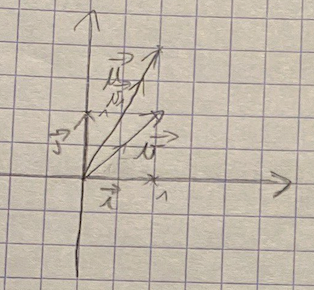
\includegraphics{../images/image01.png}\\
b) $e_1 = \begin{pmatrix}
    1\\
    0\\
\end{pmatrix}, e_2 = \begin{pmatrix}
    0\\
    1\\
\end{pmatrix}$\\
$p(e_1) = \frac{<\vec{u}|\vec{e_1}>}{<\vec{u}|\vec{u}>}\vec{u}$\\
$<\vec{u}|\vec{u}> = \left<
    \begin{pmatrix}
        1\\
        2\\
    \end{pmatrix} | \begin{pmatrix}
        1\\
        2\\
    \end{pmatrix}
\right> = 5$\\
$<\vec{e_1}|\vec{u}> = \left<
    \begin{pmatrix}
        1\\
        0\\
    \end{pmatrix} | \begin{pmatrix}
        1\\
        2\\
    \end{pmatrix}
\right> = 1$\\
$p(e_1) = \frac{1}{5} \begin{pmatrix}
    1\\
    2\\
\end{pmatrix} = \frac{1}{5} e_1 + \frac{2}{5} e_2$\\
$p(e_2) = \frac{<\vec{u}|\vec{e_2}>}{<\vec{u}|\vec{u}>}\vec{u}$\\
$<\vec{e_2}|\vec{u}> = \left<
    \begin{pmatrix}
        0\\
        1\\
    \end{pmatrix} | \begin{pmatrix}
        1\\
        2\\
    \end{pmatrix}
\right> = 2$\\
$p(e_1) = \frac{2}{5} \begin{pmatrix}
    1\\
    2\\
\end{pmatrix} = \frac{2}{5} e_1 + \frac{4}{5} e_2$\\
$P = \begin{pmatrix}
    \frac{1}{5} & & \frac{2}{5}\\
    & & \\
    \frac{2}{5} & &\frac{4}{5}\\
\end{pmatrix}$\\

\newpage

\noindent Soit $\vec{w} \in P$\\
On a que $s(w) = 2p(\vec{w}) - \vec{w}$\\
Donc $S = 2P - I_2$\\
$S = \begin{pmatrix}
    \frac{2}{5} & & \frac{4}{5}\\
    & & \\
    \frac{4}{5} & &\frac{8}{5}\\
\end{pmatrix} - \begin{pmatrix}
    1 & & 0\\
    & & \\
    0 & & 1\\
\end{pmatrix} = \begin{pmatrix}
    -\frac{3}{5} & & \frac{4}{5}\\
    & & \\
    \frac{4}{5} & & \frac{3}{5}\\
\end{pmatrix}$\\
\\
c) On a que $P^2 = P$ $\rightarrow$ projection\\  
On a que $S^2 = I_2$ $\rightarrow$ symétrie  

\end{document}